%! TEX root = ../main.tex

\section{PE формат}
Исполняемые файлы в системе Windows имеет общую сигнатуру, называемую
PE (Portable Executable). В PE формате содержится различная информация о
исполняемом файле, как например: таблицы импорта и экспорта, информация о
различных секциях, точка входа и так далее. Структура PE формата представлена на
рисунке \ref{fig:PE}.
\begin{figure}[htb]
  \centering
  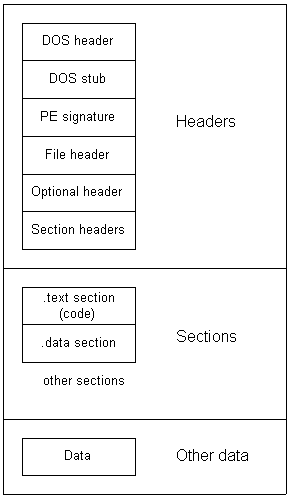
\includegraphics[width=0.45\textwidth]{PE.png}
  \caption{Формат PE}
  \label{fig:PE}
\end{figure}

Рассмотрим те части PE формата, которые будут использованы в данной работе.
Первым идет MS-DOS заголовок, первыми двумя байтами которой является сигнатура
"MZ". Большая часть полей данного заголовка предназаначены для запуска из-под
DOS. Для дальнейшей работы, кроме проверки сигнатуры, потребуется поле
\verb!e_lfanew!, в котором содержится указатель на начало PE-заголовока.

PE-заголовок также имеет свою сигнатуру, которую необходимо проверить на
корректность, а именно четыре байта "PE\textbackslash0\textbackslash0". В данном
разделе хранится количество секций \verb!NumberOfSection!, а также размер
идущего за следующим опционального заголовка в байтах
\verb!SizeOfOptionalHeader!.

Далле расположен опциональный заголовок. Данный раздел содежит смещение адреса
входа относительно базового адреса загрузки файла --- \texttt{AddresOfEntryPoint},
рекомендуемый базовый адрес загрузки файла \verb!ImageBase!, количество
элементов в таблице \verb!DATA_DIRECTORY! --- \verb!NumberOfRvaAndSizes!.
\verb!DATA_DIRECTORY! представляет собой таблицу, каждый элемент которой
представляет из себя структуру из двух полей, а именно виртулього адреса тех
данных, на который указывает данный элемент, и их размер. 

Далее идет таблица секций. Для каждой секции в этой таблице приведена следующая
информация:
\begin{itemize}
  \item \verb!Name! --- имя секции. 
  \item \verb!VirtualAddress! --- виртуальный адрес секции в памяти.
  \item \verb!PointerToRawData! --- указатель на данные в файле.
  \item \verb!VirtualSize! --- размер, занимаемый секцией в памяти.
  \item \verb!Characteristics! --- свойства секции. Так, например, секция,
    которую можно запустить на выполнение должна обладать свойством
    \verb!IMAGE_SCN_CNT_CODE!.
\end{itemize}
